%% Springer Nature article version of the manuscript.
%% The original Elsevier source remains in pi_cda_paper.tex.
\documentclass[pdflatex,sn-mathphys-num]{sn-jnl}

\usepackage{amsmath,amssymb,amsfonts}
\usepackage{graphicx}
\usepackage{textcomp}
\usepackage{xcolor}
\usepackage{booktabs}
\usepackage{multirow}
\usepackage{float}
\usepackage{url}
\usepackage{acronym}
\usepackage[section]{placeins}

\hypersetup{hidelinks}
\raggedbottom
\providecommand{\burl}[1]{\url{#1}}

\acrodef{hrc}[HRC]{Human-Robot Collaboration}
\acrodef{dt}[DT]{Digital Twin}
\acrodef{uda}[UDA]{Unsupervised Domain Adaptation}
\acrodef{ctrgcn}[CTR-GCN]{Channel-wise Topology Refinement Graph Convolutional Network}
\acrodef{stgcn}[ST-GCN]{Spatial-Temporal Graph Convolutional Network}
\acrodef{tcmmd}[TC-MMD]{Topology-Consistent Maximum Mean Discrepancy}
\acrodef{mmd}[MMD]{Maximum Mean Discrepancy}
\acrodef{dann}[DANN]{Domain-Adversarial Neural Network}
\acrodef{coral}[CORAL]{Correlation Alignment}
\acrodef{mocap}[MoCap]{Motion Capture}
\acrodef{vr}[VR]{Virtual Reality}
\acrodef{f1}[F1]{F1-score}
\acrodef{bvh}[BVH]{Biovision Hierarchy}
\acrodef{acc}[ACC]{Accuracy}
\acrodef{fm}[FM]{FixMatch}
\acrodef{auc}[AUC]{Area Under the Receiver Operating Characteristic Curve}
\acrodef{em}[EM]{Expectation-Maximisation}
\acrodef{inhard}[InHARD]{Industrial Human Action Recognition Dataset}
\acrodef{inharddt}[InHARD-DT]{Industrial Human Action Recognition Dataset Digital Twin}

\begin{document}

\title{Digital-Twin Pretraining for Label-Efficient Skeleton Action Recognition in Industrial Workcells}

% \author[1,2]{\fnm{Ameur} \sur{Gargouri}}
% \author*[2]{\fnm{Mohamed} \sur{Karray}}\email{mohamed.karray@esme.fr}
% \author[1]{\fnm{Mohamed} \sur{Ksantini}}

% \affil[1]{\orgdiv{ATISP Lab}, \orgname{ENET'Com, University of Sfax},
%   \orgaddress{\city{Sfax}, \country{Tunisia}}}
% \affil[2]{\orgname{ESME Research Lab},
%   \orgaddress{\city{Ivry-sur-Seine}, \country{France}}}

\abstract{%
  In industrial settings, a recognition system must identify workers' actions
  across different workcells, yet collecting and annotating physical recordings
  for every worker, object configuration, and execution style is costly. A
  digital twin can provide labelled skeleton sequences in a controllable virtual
  source domain, but those sequences differ from physical target-domain
  recordings in posture, timing, object interaction, and workcell context, and
  it remains unclear whether a recogniser trained on them transfers to unseen
  physical workers and how much target supervision it still needs. In this
  work, we propose a label-efficient strategy that trains on the twin and a few
  labelled physical clips with a class-prototype term, then fine-tunes. The
  evaluation covers virtual-to-physical transfer between the digital twin version and
  the     physical one of the Industrial Human Action Recognition Dataset (InHARD-DT and InHARD respectively) with a common CTR-GCN backbone, four
  subject-disjoint target folds, and three random seeds. Without target labels,
  source-only transfer reaches $40.59\pm2.93\%$ macro-F1, and none of five
  unsupervised adaptation strategies improves on it, with TC-MMD at
  $39.34\pm2.50\%$. With target labels, a model initialised
  on the digital twin matches the macro-F1 of a model trained on physical clips
  alone while using five to twenty times fewer labelled clips. The
  class-prototype objective adds a significant gain at one and five clips per
  class, and the proposed strategy reaches
  $66.27\pm3.46\%$ macro-F1 using 50 labelled clips per class, versus
  $75.22\pm4.04\%$ for the target-supervised oracle.
}

\keywords{human-robot collaboration, digital twin, skeleton action recognition,
  sim-to-real transfer, label efficiency, domain adaptation, industrial workcells}

\maketitle

\section*{Article Highlights}
\begin{itemize}
  \item Digital twin recordings cut the physical clips needed to train skeleton action recognition in industrial workcells.
  \item Training on twin data together with a few labelled physical clips helps most when physical labels are scarce.
  \item Unlabelled domain adaptation alone does not close the gap between virtual and physical assembly work.
  \item Virtual and physical workers differ in posture, timing and object handling rather than in sensor noise.
  \item Label-efficient recognition helps collaborative robots follow worker actions with little annotation effort.
\end{itemize}

\section{Introduction}
\label{sec:introduction}

A robot that shares an assembly cell with a person must recognise what that
person is doing in order to offer a part, prepare a tool or keep a safe
distance~\cite{wang2018hrcmotion}. Skeleton sequences suit this task because
they are compact, less privacy-invasive than video and directly encode the body
configuration that distinguishes manipulation actions, and graph convolutional
recognisers built on them are now the reference approach for skeleton action
recognition~\cite{yan2018stgcn,chen2021ctrgcn,liu2025skeletonreview}. These
recognisers are trained on large labelled corpora such as NTU
RGB+D~\cite{shahroudy2016ntu,liu2020ntu120}, whereas an industrial deployment
needs labelled sequences for the specific workstation, its objects and its
workers. Recording and annotating them on a running line is slow, costly and
interrupts production.

Digital twins offer a way around this cost~\cite{tao2019digitaltwin}. A
virtual-reality replica of a workstation lets participants perform the assembly
procedure while every action is labelled automatically, and
\ac{inharddt}~\cite{dallel2023digital} provides such a replica of the physical
\ac{inhard} workstation~\cite{dallel2020inhardpaper}. Virtual execution
nevertheless differs from physical work. Virtual parts carry no weight and
offer no contact, the workstation is reached through a headset, and the
recorded segments are cut by the generator rather than by an annotator. Whether
a model trained on such data works for real workers, and how many physical
labels it still needs, determines whether a digital twin reduces the
commissioning effort of a collaborative cell at all.

This paper measures both quantities under a protocol that keeps physical test
workers unseen by every training and adaptation step. We first evaluate
zero-shot transfer from \ac{inharddt} to \ac{inhard} with source-only
training and five unsupervised adaptation methods, then explain the observed
gap through kinematic descriptors and targeted interventions, and finally
measure how much the digital twin reduces the number of physical labels needed
when a small labelled calibration set can be collected. The contribution is
fourfold in content but forms a single argument. It provides a reproducible
real-data benchmark for virtual-to-physical skeleton action recognition with a
fixed \ac{ctrgcn} backbone, four subject-disjoint target folds and three
seeds, extending the original \ac{inharddt} study~\cite{dallel2023digital}.
It shows that distribution alignment, pseudo-labelling and a
topology-consistent alignment variant do not improve on source-only transfer,
and that adversarial alignment degrades it significantly. It explains this
failure through a gap analysis which rules out sensor noise, class-prior shift,
generator segmentation and bimanual behaviour as dominant causes and points
instead to class-conditional execution differences. Finally, it quantifies the
practical value of the twin as a five- to twenty-fold reduction in physical
labels across budgets from one to fifty clips per class, and shows that joint
twin and physical training with a class-prototype alignment term is the best
strategy when labels are scarcest.

\section{Related Work}
\label{sec:related}

Skeleton action recognition moved from hand-crafted joint features to graph
convolutional networks that treat joints as nodes and bones as edges. The
\ac{stgcn} of Yan et al.~\cite{yan2018stgcn} introduced spatial-temporal graph
convolution on a fixed body graph, and \ac{ctrgcn}~\cite{chen2021ctrgcn}
refines that graph per channel and per sample, which made it a standard
backbone on NTU RGB+D~\cite{shahroudy2016ntu,liu2020ntu120}. Later work models
heterogeneous skeletons with different joint sets~\cite{wang2025heterogeneous}
and higher-order joint relations through hypergraphs~\cite{chen2025hypergraph},
and a recent review covers representation, temporal modelling and evaluation
practice~\cite{liu2025skeletonreview}. In manufacturing, deep motion
recognition has been used to anticipate worker needs in collaborative
assembly~\cite{wang2018hrcmotion}. We keep the \ac{ctrgcn} backbone fixed so
that differences between experiments reflect the transfer strategy rather than
model capacity.

Digital twins are virtual counterparts of physical production assets that are
increasingly used for design, monitoring and training data
generation~\cite{tao2019digitaltwin}. Human-centred engineering already uses
virtual reality to prototype workstations and interfaces with
users~\cite{valentini2025digital}. For perception, simulation-based training
must cross a reality gap, which robotics has addressed with domain
randomisation~\cite{tobin2017domainrandomization} and with careful evaluation
of simulated policies on the physical task~\cite{rothert2024simtoreal}. Dallel
et al. released \ac{inhard}~\cite{dallel2020inhardpaper,dallel2020inhard} and
its virtual replica \ac{inharddt}~\cite{dallel2023digital,dallel2023dataset},
and reported an \ac{stgcn} trained on the twin and tested on physical data.
Our study differs in its strictly subject-disjoint folds, its multi-seed
statistics, its explanation of the gap and its measurement of label savings.
Because the backbone and protocol differ, their published figure serves as
context and not as a paired baseline.

Unsupervised domain adaptation trains on labelled source data and unlabelled
target data, with theory bounding the target error by the source error plus a
divergence between domains~\cite{bendavid2010theory}. Common instantiations
minimise a multi-kernel \ac{mmd}~\cite{long2015dan}, match second-order
statistics~\cite{sun2016deepcoral} or learn domain-invariant features
adversarially~\cite{ganin2016dann}. Zhao et al.~\cite{zhao2019invariant} showed
that invariant marginal representations cannot guarantee transfer when the
class-conditional distributions or the label distributions differ, and prior
shift alone can be corrected by re-estimating class priors with an
\ac{em} procedure~\cite{saerens2002priors}. For skeletons, temporal
adaptation has been studied between capture setups~\cite{tian2024temporaladaptation},
graph-based adaptation has been applied to wearable sensors~\cite{yang2024domainhar},
and physics-informed constraints have been added to adaptation in industrial
diagnosis~\cite{he2024physicsinformed}. Our topology-consistent variant tests
the analogous idea of constraining skeleton graph structure during alignment.

When a few target labels exist, semi-supervised learning and semi-supervised
domain adaptation become applicable. FixMatch~\cite{sohn2020fixmatch} trains on
confident pseudo-labels from weakly augmented views, minimax
entropy~\cite{saito2019mme} adapts a prototype-based classifier with a handful
of labelled target samples, and prototypical networks~\cite{snell2017prototypical}
represent each class by the mean of its embedded examples. For skeletons,
cross-sample feature aggregation~\cite{zhang2025skeletonx} and cross-modal
contrastive pretraining~\cite{lu2024crossmodalfewshot} improve recognition from
scarce labels. We adopt the semi-supervised adaptation setting with a digital
twin as the labelled source and measure the label budget at which its benefit
appears and fades.

\section{Methodology}
\label{sec:methodology}

Figure~\ref{fig:methodology} summarises the evaluation, from the two datasets
through shared preprocessing and the transfer strategies to testing on held-out
physical workers.

\begin{figure}[!t]
  \centering
  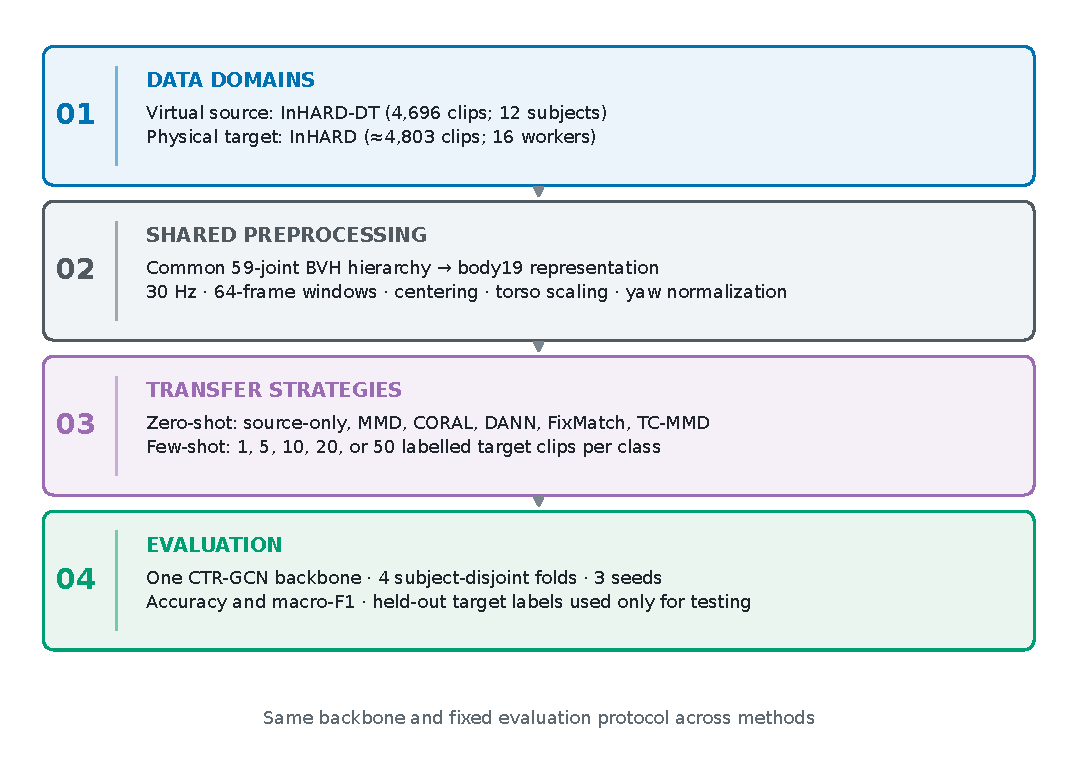
\includegraphics[width=0.9\textwidth]{figures/paper_ready/methodology.pdf}
  \caption{Evaluation workflow from paired datasets to held-out workers.}
  \label{fig:methodology}
\end{figure}

\subsection{Problem formulation}

Let $\mathcal{S}=\{(x_i^s,y_i^s)\}_{i=1}^{n_s}$ denote labelled skeleton clips
from the digital twin and $\mathcal{T}=\{x_j^t\}_{j=1}^{n_t}$ unlabelled clips
from the physical workcell, with labels $y\in\{1,\dots,C\}$ over $C=13$
actions. A recogniser $f_\theta=h\circ g$ consists of an encoder $g$ that maps
a clip to a feature vector $z=g(x)\in\mathbb{R}^{256}$ and a linear classifier
$h$. In the zero-shot setting $f_\theta$ is learned from $\mathcal{S}$ and
$\mathcal{T}$ only. In the label-efficient setting a support set
$\mathcal{T}^{\ell}_{k}$ with $k$ labelled physical clips per class is also
available. In both settings the evaluation workers are disjoint from every
worker used for training or adaptation.

\subsection{Datasets}

\ac{inharddt} contains 4,696 segmented clips from 12 participants recorded in
26 sessions while they performed the assembly procedure in a virtual replica
of the workstation~\cite{dallel2023digital,dallel2023dataset}. \ac{inhard}
contains 4,803 clips from 16 workers at the physical
workstation~\cite{dallel2020inhardpaper,dallel2020inhard}, after the removal of
the 500 ``No action'' clips that have no virtual counterpart. Both datasets were
captured with a Perception Neuron inertial \ac{mocap} suit, share the same
59-joint \ac{bvh} hierarchy at about 119 Hz and use the same 13 meso-level
action classes. The transfer problem is therefore one of physical context,
worker population and execution, not of sensor modality.
Figure~\ref{fig:dataset-collection} reproduces the original capture setups
under the Creative Commons Attribution 4.0 International
licence~\cite{dallel2023dataset,dallel2020inhard}.

\begin{figure}[!t]
  \centering
  \begin{minipage}[t]{0.485\linewidth}
    \vspace{0pt}\centering
    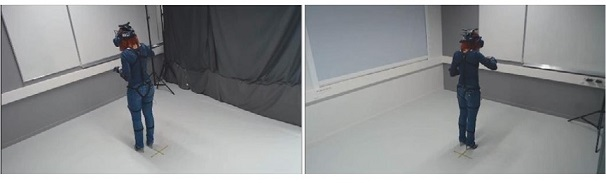
\includegraphics[width=\linewidth]{figures/dataset_collection/inhard_dt_vr_capture.jpg}
  \end{minipage}\hfill
  \begin{minipage}[t]{0.485\linewidth}
    \vspace{0pt}\centering
    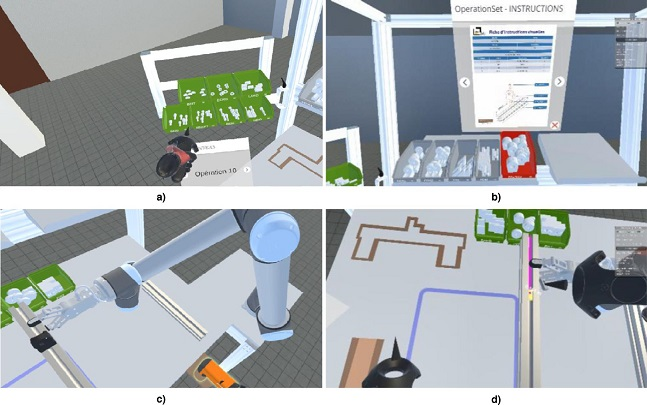
\includegraphics[width= \linewidth]{figures/dataset_collection/inhard_dt_workstation_views.jpg}
  \end{minipage}
  \par\smallskip
  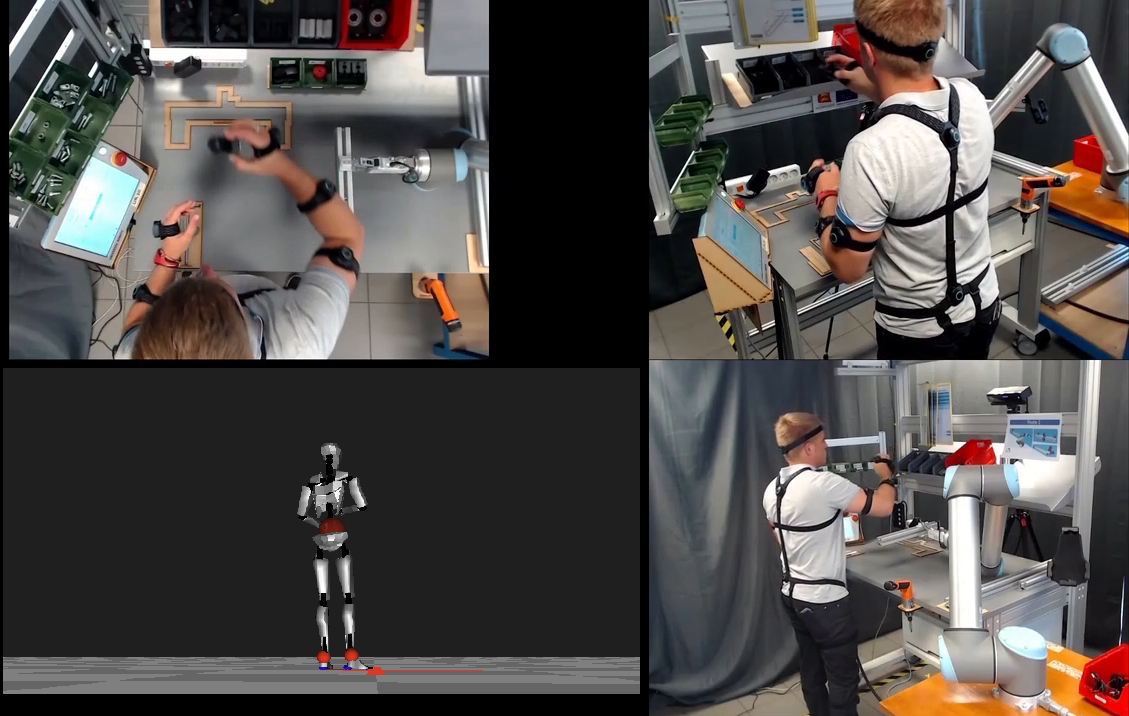
\includegraphics[width=0.5\linewidth]{figures/dataset_collection/inhard_physical_capture.png}
  \caption{Virtual and physical capture setups of the two datasets.}
  \label{fig:dataset-collection}
\end{figure}

\subsection{Preprocessing}

Each \ac{bvh} clip is converted to world joint positions by forward
kinematics and resampled to 30 Hz. We retain 19 joints that cover the hips,
spine, neck, head, both shoulders, elbows and wrists, a knuckle on each hand to
encode hand orientation, and both hips, knees and ankles. Each clip is then
canonicalised by subtracting the hip position of its first frame, rotating it
about the vertical axis so that the first-frame hip line is aligned with a
fixed direction, and dividing by the mean hip-to-neck distance. The rotation
step matters here because the two workstations face nearly opposite world
directions, as Section~\ref{sec:gap} shows. Clips are resampled to 64 frames
before entering the network. None of these steps uses labels or test-worker
information, and both domains pass through the same pipeline.

\subsection{Evaluation protocol}

The 16 \ac{inhard} workers are split into four fixed folds of four workers.
For each fold, the remaining 12 workers form the target adaptation pool, which
supplies unlabelled clips for unsupervised adaptation and the labelled support
set in the label-efficient setting, while the four held-out workers are used
only for testing. All \ac{inharddt} participants form the source domain. Every
experiment is repeated with three seeds, so each reported mean and standard
deviation covers 12 fold-seed runs. Training length is fixed in advance and
the final weights are evaluated, so target labels never influence model
selection. We report \ac{acc} and macro-\ac{f1}, the latter being the primary
metric because the 13 classes are imbalanced and unequal in difficulty. Paired
comparisons use a two-sided Wilcoxon signed-rank test over the 16 physical
workers, each represented by its seed-averaged macro-\ac{f1} computed from the
predictions of the fold in which it was held out. The $p$-values are not
corrected for multiple comparisons and should be read as exploratory.

\subsection{Common recogniser and training}

All methods share the same \ac{ctrgcn} encoder~\cite{chen2021ctrgcn}, built
from ten units of 64, 128 and 256 channels that each combine a channel-wise
refined graph convolution with multi-scale temporal convolutions. For an input
feature map $\mathbf{X}\in\mathbb{R}^{C\times T\times V}$ over $T$ frames and
$V=19$ joints, the graph convolution computes output channel $c$ as
\begin{equation}
  \mathbf{Z}_c=\sum_{g=1}^{G}\bigl(\mathbf{A}_g+\alpha\,\mathbf{Q}_{g,c}\bigr)\,
  \bigl(\mathbf{X}\mathbf{W}_g\bigr)_c,\qquad
  \mathbf{Q}_{g}=\xi_g\Bigl(\tanh\bigl(\phi_g(\bar{\mathbf{X}})_u-\psi_g(\bar{\mathbf{X}})_v\bigr)\Bigr),
  \label{eq:ctrgc}
\end{equation}
where $\mathbf{A}_g$ is the normalised skeleton adjacency of subset $g$ among
the self, inward and outward subsets, $\bar{\mathbf{X}}$ is the temporal mean
of $\mathbf{X}$, $\phi_g$, $\psi_g$ and $\xi_g$ are $1\times1$ convolutions and
$\alpha$ is a learned scalar. Each channel therefore aggregates joints through
the shared skeleton graph corrected by a sample-specific topology, which lets
the encoder model hand and arm coordination that the anatomical graph does not
connect directly.

The encoder output is averaged over time and joints into $z=g(x)$ and
classified by $p_\theta(\cdot\mid x)=\mathrm{softmax}\bigl(h(z)\bigr)$. Every
supervised model minimises the cross-entropy over a labelled set $\mathcal{D}$,
\begin{equation}
  \mathcal{L}_{\mathrm{CE}}(\mathcal{D})=-\frac{1}{|\mathcal{D}|}
  \sum_{(x,y)\in\mathcal{D}}\log p_\theta(y\mid x),
  \label{eq:ce}
\end{equation}
and the supervised references differ only in that set. The source-only model
uses $\mathcal{D}=\mathcal{S}$, the target oracle uses the labelled 12-worker
pool $\mathcal{T}^{\ell}$, the source-plus-target model uses
$\mathcal{S}\cup\mathcal{T}^{\ell}$, and the digital-twin in-domain model uses
\acs{inharddt} participants disjoint from its test participants, which gives
the level that the source domain itself supports.

Optimisation uses stochastic gradient descent with Nesterov momentum $0.9$,
weight decay $4\times10^{-4}$ and batch size 64 for 50 epochs. After five
linear warm-up epochs, the learning rate at step $t$ of $T_{\max}$ follows
\begin{equation}
  \eta_t=\frac{\eta_0}{2}\Bigl(1+\cos\frac{\pi\,(t-t_w)}{T_{\max}-t_w}\Bigr),
  \label{eq:lr}
\end{equation}
with $\eta_0=0.05$ and $t_w$ the last warm-up step, so that every method
receives the same training budget. Training clips are mildly augmented by
temporal cropping to 85--100\% of their length, rotation of up to $10^\circ$
about the vertical axis and scaling by up to 5\%.

\subsection{Unsupervised adaptation objectives}

Each unsupervised method adds an alignment term to the source cross-entropy and
optimises, on mini-batches $\mathcal{B}_s$ and $\mathcal{B}_t$ of 64 source and
64 unlabelled target clips,
\begin{equation}
  \mathcal{L}=\mathcal{L}_{\mathrm{CE}}(\mathcal{B}_s)
  +\lambda\,\mathcal{L}_{\mathrm{align}}(\mathcal{B}_s,\mathcal{B}_t).
  \label{eq:uda}
\end{equation}
The methods differ in $\mathcal{L}_{\mathrm{align}}$, that is in which property
of the two feature distributions they force to agree.

\ac{mmd}~\cite{long2015dan} compares the source and target feature
distributions through their mean embeddings in a kernel space,
\begin{equation}
  \mathcal{L}_{\mathrm{MMD}}=\frac{1}{n_s^2}\sum_{i,i'}k(z_i^s,z_{i'}^s)
  +\frac{1}{n_t^2}\sum_{j,j'}k(z_j^t,z_{j'}^t)
  -\frac{2}{n_sn_t}\sum_{i,j}k(z_i^s,z_j^t),\qquad
  k(z,z')=\sum_{q=0}^{4}\exp\Bigl(-\frac{\|z-z'\|^2}{2^{\,q-2}\,\bar{d}}\Bigr),
  \label{eq:mmd}
\end{equation}
where $\bar{d}$ is the mean pairwise squared distance in the batch. The mixture
of five bandwidths makes the term sensitive to differences at several scales,
and it is weighted by $\lambda=0.5$.

\ac{coral}~\cite{sun2016deepcoral} aligns only second-order statistics,
\begin{equation}
  \mathcal{L}_{\mathrm{CORAL}}=\frac{1}{4d^2}\bigl\|\Sigma_s-\Sigma_t\bigr\|_F^2,
  \label{eq:coral}
\end{equation}
where $\Sigma_s$ and $\Sigma_t$ are the covariance matrices of the
$d=256$-dimensional source and target features. It assumes that matching the
correlation structure of the features suffices for transfer, and it is weighted
by $\lambda=1$.

\ac{dann}~\cite{ganin2016dann} learns domain invariance adversarially. A
three-layer discriminator $D$ predicts the domain label $d_i$, equal to one for
target clips, from features passed through a gradient reversal layer
$R_\eta$,
\begin{equation}
  \mathcal{L}_{\mathrm{DANN}}=-\frac{1}{n}\sum_{i=1}^{n}
  \Bigl[d_i\log D\bigl(R_\eta(z_i)\bigr)+(1-d_i)\log\Bigl(1-D\bigl(R_\eta(z_i)\bigr)\Bigr)\Bigr],
  \qquad\eta=\frac{2}{1+e^{-10p}}-1,
  \label{eq:dann}
\end{equation}
where $R_\eta$ is the identity in the forward pass and multiplies the gradient
by $-\eta$ in the backward pass. The discriminator thus learns to separate the
domains while the encoder learns to confuse it, with a reversal strength that
grows with training progress $p\in[0,1]$, and the term is weighted by
$\lambda=1$.

\ac{fm}~\cite{sohn2020fixmatch} replaces distribution matching by
self-training on confident target predictions,
\begin{equation}
  \mathcal{L}_{\mathrm{FM}}=\frac{1}{n_t}\sum_{j=1}^{n_t}
  \mathbb{1}\Bigl[\max_c p_\theta\bigl(c\mid a(x_j^t)\bigr)\ge\tau\Bigr]\,
  \Bigl(-\log p_\theta\bigl(\hat{y}_j\mid A(x_j^t)\bigr)\Bigr),\qquad
  \hat{y}_j=\arg\max_c p_\theta\bigl(c\mid a(x_j^t)\bigr),
  \label{eq:fm}
\end{equation}
where $a$ is the weak augmentation of training, $A$ a strong augmentation with
cropping to 50--100\%, rotation up to $30^\circ$, tilt up to $10^\circ$,
scaling by up to 20\% and joint jitter, and $\tau=0.9$. A pseudo-label is used
only when the weakly augmented view is predicted confidently, and the model
then has to reproduce it on the strongly augmented view. \ac{fm} starts from
the source-only model and runs 30 epochs at learning rate $0.01$ with
$\lambda=1$.

The topology-consistent variant \ac{tcmmd} extends Eq.~\ref{eq:mmd} with a
constraint on the refined graphs of Eq.~\ref{eq:ctrgc}. With
$\bar{M}^{(l,g)}_s$ and $\bar{M}^{(l,g)}_t$ denoting the source and target
batch means of the channel-averaged refined adjacency
$\mathbf{A}_g+\alpha\mathbf{Q}_{g,c}$ in layer $l$, it minimises
\begin{equation}
  \mathcal{L}_{\mathrm{TC}}=\lambda_{\mathrm{MMD}}\mathcal{L}_{\mathrm{MMD}}
  +\frac{\lambda_{\mathrm{topo}}}{LG}\sum_{l=1}^{L}\sum_{g=1}^{G}
  \bigl\|\bar{M}^{(l,g)}_s-\bar{M}^{(l,g)}_t\bigr\|_F^2,
  \label{eq:tc}
\end{equation}
with $\lambda_{\mathrm{MMD}}=0.5$, $\lambda_{\mathrm{topo}}=0.1$, $L=10$ and
$G=3$. It encodes the hypothesis that virtual and physical workers should
coordinate their joints through the same skeletal structure, and it corresponds
to an earlier physics-informed proposal of ours that we evaluate here as one
hypothesis among others.

\subsection{Label-efficient strategies}

For each $k\in\{1,5,10,20,50\}$ the support set is drawn without replacement
within each class from the 12-worker adaptation pool, with the sampling seed
$1000s+10f+k$ for experiment seed $s$ and fold $f$. Classes with fewer than $k$
clips in the pool contribute all of them. The selected clip identifiers are
stored with every result. Seven strategies use the same support set. Training
from scratch fits a randomly initialised \ac{ctrgcn} on the support set alone,
while source-only fine-tuning and \ac{tcmmd} fine-tuning start from the
corresponding zero-shot models. These three strategies run 300 steps on the
support set at learning rates $0.05$, $0.01$ and $0.01$ respectively. The
joint strategy starts from the source-only model and trains for 30 epochs at
learning rate $0.01$ on batches that combine 64 source clips with up to 32
support clips, so that the twin keeps regularising the representation while
the physical labels correct it. Joint training with \ac{fm} adds the
pseudo-label term on unlabelled clips of the adaptation pool. Joint training
with a prototype term adds a class-conditional alignment inspired by
prototypical networks~\cite{snell2017prototypical}. With $\hat{z}=z/\|z\|$,
$\mu_c^s$ and $\mu_c^\ell$ the batch means of $\hat{z}$ over source clips and
support clips of class $c$, and $\mathcal{C}_b$ the classes present in both
parts of the batch, it adds
\begin{equation}
  \mathcal{L}_{\mathrm{proto}}=\frac{1}{|\mathcal{C}_b|}\sum_{c\in\mathcal{C}_b}
  \bigl\|\mu_c^s-\mu_c^\ell\bigr\|_2^2
  \label{eq:proto}
\end{equation}
with weight one to the joint cross-entropy. Unlike Eq.~\ref{eq:mmd}, this term
aligns each class separately and therefore addresses class-conditional shift.
The last strategy follows this joint prototype training with 300 steps of
fine-tuning on the support set alone at learning rate $0.01$. No
hyperparameter was tuned on the held-out workers.

\subsection{Gap analysis}

To explain the transfer gap we describe every clip by 17 kinematic descriptors
computed in world or canonical coordinates. They cover clip duration, the
first-frame facing direction, hip displacement and path length, mean and peak
wrist speed, the share of hand motion carried by the right hand, hand height
and reach relative to the torso, trunk flexion, elbow angle ranges, head
height, the log dimensionless jerk of the right wrist as a smoothness
measure~\cite{balasubramanian2015smoothness}, and the share and absolute power
of wrist velocity above 4 Hz as a jitter proxy. Domain differences are tested
with Mann-Whitney U tests, Benjamini-Hochberg correction and Cliff's delta as
the effect size, globally and per class. A gradient-boosting domain classifier
trained on the descriptors with five-fold cross-validation grouped by subject
measures how separable the domains are. We then test three candidate causes by
intervention on the source-only model of seed 0. Prior shift is tested by
re-weighting its posteriors with the target class prior, both estimated with
the \ac{em} procedure of Saerens et al.~\cite{saerens2002priors} from the
unlabelled adaptation pool and taken as the true prior of that pool as an upper
bound. Segmentation artefacts are tested by retraining with random sub-windows
covering 30--100\% of every source clip. Bimanual behaviour is tested by
removing left-arm motion relative to the shoulder, at test time only and at
both training and test time.

\section{Results}
\label{sec:results}

\subsection{Zero-shot transfer}

Table~\ref{tab:main} compares the in-domain reference, source-only transfer,
five unsupervised adaptation methods and the two target-supervised controls.

\begin{table}[!t]
  \centering
  \caption{Zero-shot transfer and supervised controls over 12 runs.}
  \label{tab:main}
  \small
  \begin{tabular}{lrr}
    \toprule
    Method             & \ac{acc} (\%)           & Macro-\ac{f1} (\%)      \\
    \midrule
    \ac{dt} in-domain  & $75.47\pm3.54$          & $73.32\pm4.04$          \\
    \midrule
    Source-only        & $50.16\pm2.97$          & $\mathbf{40.59\pm2.93}$ \\
    \ac{dann}          & $46.71\pm3.89$          & $38.17\pm3.00$          \\
    \ac{coral}         & $48.17\pm4.00$          & $38.88\pm3.10$          \\
    \ac{mmd}           & $49.21\pm3.18$          & $39.66\pm3.00$          \\
    \ac{tcmmd}         & $48.35\pm2.79$          & $39.34\pm2.50$          \\
    \ac{fm}            & $50.75\pm2.91$          & $40.54\pm2.93$          \\
    \midrule
    Target oracle      & $82.67\pm2.38$          & $75.22\pm4.04$          \\
    Source plus target & $\mathbf{83.95\pm1.98}$ & $\mathbf{75.89\pm3.20}$ \\
    \bottomrule
  \end{tabular}
\end{table}

A recogniser trained on the digital twin reaches $73.32\%$ macro-\ac{f1} on
unseen virtual participants but only $40.59\%$ on unseen physical workers,
while the target oracle reaches $75.22\%$. The twin therefore supports a
recogniser as accurate as one trained on physical labels, yet that recogniser
loses about 35 points when it meets physical work. None of the unsupervised
methods narrows this gap. \ac{fm} matches source-only transfer at $40.54\%$,
with a subject-level difference of $+0.21$ points at $p=0.82$, and the
alignment methods all fall below it. \ac{mmd} and \ac{tcmmd} lose $0.93$ and
$1.25$ points of mean macro-\ac{f1}, with subject-level $p$-values of $0.63$
and $0.10$, and \ac{dann} loses $2.42$ points, which is significant across the
16 workers at $p=0.001$. The topology term of \ac{tcmmd} brings no benefit over
plain \ac{mmd}. When physical labels are available, adding the twin to the
labelled pool raises mean macro-\ac{f1} from $75.22\%$ to $75.89\%$, a
difference that is not significant at $p=0.43$. Class-level scores show where
transfer breaks down: source-only transfer recognises \emph{Picking left} at
$77.1\%$ \ac{f1} but \emph{Consult sheets}, \emph{Take component} and
\emph{Take subsystem} only at $12.5\%$, $18.8\%$ and $16.4\%$, where the oracle
reaches $30.6\%$, $74.5\%$ and $60.8\%$. Figure~\ref{fig:zeroshot} visualises
these comparisons.

\begin{figure}[!t]
  \centering
  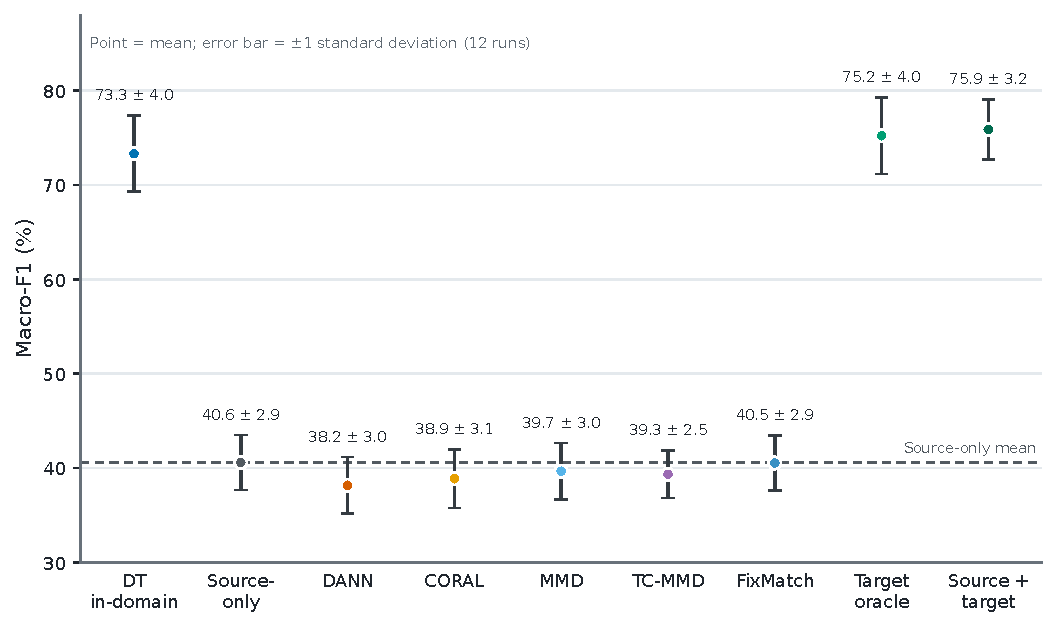
\includegraphics[width=.92\textwidth]{figures/paper_ready/zero_shot.pdf}
  \caption{Macro-F1 of zero-shot transfer and supervised controls.}
  \label{fig:zeroshot}
\end{figure}

\subsection{Characterising the virtual-to-physical gap}
\label{sec:gap}

The descriptors separate the two domains almost perfectly. The grouped domain
classifier reaches an \ac{auc} of $1.00$ with all descriptors and still
$0.97$ without the facing direction, and duration alone gives $0.87$. The most
extreme difference is the facing direction, with median first-frame headings
of $-59.5^\circ$ for \ac{inharddt} and $109.5^\circ$ for \ac{inhard}, as the
upper two panels of Figure~\ref{fig:gap} show. This difference of about $170^\circ$
reflects how the two workstations are oriented in their world frames, and the
yaw normalisation of the preprocessing removes it before training.

\begin{figure}[!t]
  \centering
  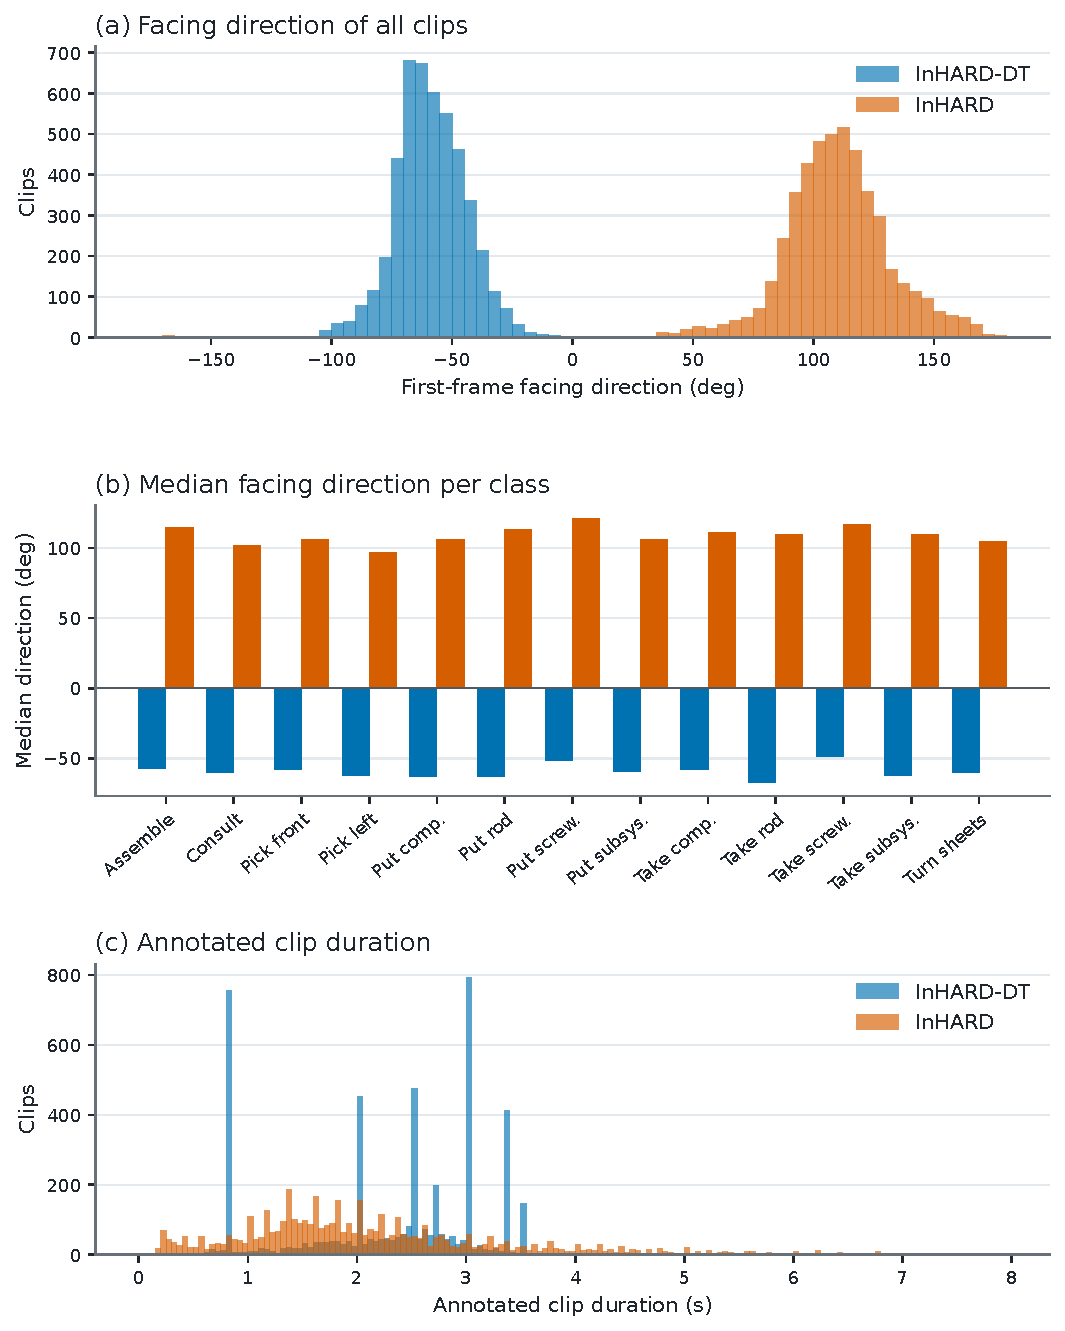
\includegraphics[width=0.8\textwidth]{figures/paper_ready/gap.pdf}
  \caption{Facing direction and annotated clip duration in both domains.}
  \label{fig:gap}
\end{figure}

The lower panel of Figure~\ref{fig:gap} reveals a segmentation artefact. Five
durations of $3.0$, $0.8$, $2.5$, $2.0$ and $3.4$ seconds account for $58.1\%$
of all \ac{inharddt} clips, against $10.0\%$ for the five most frequent
durations of \ac{inhard}. The generator cuts fixed windows around virtual
events for short actions, so $97$ to $99\%$ of \emph{Take subsystem},
\emph{Take component} and \emph{Put down component} clips have identical
lengths, whereas \emph{Assemble system}, \emph{Consult sheets} and both
long put-down actions keep natural boundaries. Durations of the virtual clips
therefore reflect annotation rather than execution speed. The behaviour of the
workers also differs. Physical workers use the left arm more, with a median
left elbow range of $15.0^\circ$ against $8.3^\circ$ in the twin, and the
difference reaches $27.5^\circ$ against $3.1^\circ$ for \emph{Take component},
while the right hand carries $62\%$ of hand motion in the twin against $55\%$
at the physical workstation. Class proportions differ as well:
\emph{Assemble system} makes up $11.0\%$ of virtual clips and $28.7\%$ of
physical clips, whereas \emph{Take subsystem} falls from $7.1\%$ to $0.8\%$.
Physical recordings also carry more high-frequency motion. Absolute wrist
velocity power above 4 Hz is $2.7$ to $2.8$ times higher than in the twin, and
the hips, spine, head and feet show ratios between $1.6$ and $2.6$, which
indicates a body-wide sensor component together with additional hand
activity. The magnitude of this excess corresponds to position fluctuations
below $2$ mm, far smaller than the centimetre-scale motion that distinguishes
the actions. A gradient-boosting classifier on the same descriptors confirms
how hard the transfer is: trained on the twin it reaches $18.2\%$
macro-\ac{f1} on physical clips, against $52.6\%$ when trained and tested on
disjoint physical workers.

The interventions show which of these differences limit the recogniser.
Re-weighting the source-only posteriors with the true class prior of the
adaptation pool changes macro-\ac{f1} from $41.37\%$ to $41.47\%$ on seed 0,
and the \ac{em} estimate of that prior lowers it to $39.01\%$ because the
estimate itself is biased, placing $16.6\%$ of the mass on
\emph{Consult sheets} in the first fold whose true share is $2.1\%$. Class-prior shift is
therefore real but not the limiting factor. Random sub-window training lowers
macro-\ac{f1} to $36.88\%$: it helps \emph{Take subsystem}, from $16.1\%$ to
$25.8\%$ \ac{f1}, but cuts the short fixed-window actions, with
\emph{Put down component} falling from $67.7\%$ to $40.0\%$, because a
0.8-second window contains the whole action. Removing left-arm motion lowers
macro-\ac{f1} to $31.01\%$ when applied at test time and to $30.46\%$ when
applied during training as well, and \emph{Picking left} falls from $78.3\%$
to $49.1\%$, so the left arm carries discriminative information rather than
noise. None of the candidate causes accounts for the gap. The remaining
explanation, consistent with the class-level results above, is that each
action is executed differently with real parts and tools than with virtual
ones. This class-conditional shift is precisely the situation in which
marginal alignment cannot be expected to help~\cite{zhao2019invariant}, which
explains the results of Table~\ref{tab:main}.

\subsection{Label efficiency of digital-twin pretraining}
\label{sec:label-budget}

Table~\ref{tab:fewshot} reports macro-\ac{f1} for the seven strategies at the
five label budgets. Training from scratch on physical labels is the reference
for what the labels achieve without the twin, and source-only fine-tuning is
the reference against which the significance markers are computed.

\begin{table}[!t]
  \centering
  \caption{Macro-F1 in \% by strategy and labelled clips per class.}
  \label{tab:fewshot}
  \small
  \setlength{\tabcolsep}{3pt}
  \begin{tabular}{lccccc}
    \toprule
    Strategy                         & $k=1$                              & $k=5$                       & $k=10$                  & $k=20$                  & $k=50$                  \\
    \midrule
    Scratch                          & $11.36\pm3.18^{-}$                 & $22.46\pm2.97^{-}$          & $34.08\pm2.92^{-}$      & $42.77\pm3.56^{-}$      & $51.39\pm4.50^{-}$      \\
    Source-only fine-tuning          & $29.28\pm6.06$                     & $45.64\pm3.81$              & $53.10\pm3.80$          & $59.11\pm2.98$          & $64.99\pm3.11$          \\
    \ac{tcmmd} fine-tuning           & $31.25\pm5.48$                     & $43.95\pm3.74^{-}$          & $52.55\pm2.10$          & $58.40\pm2.64$          & $64.88\pm2.89$          \\
    Joint                            & $42.50\pm4.09^{+}$                 & $48.43\pm4.04^{+}$          & $52.54\pm3.51$          & $57.06\pm3.60^{-}$      & $61.85\pm3.88^{-}$      \\
    Joint with \ac{fm}               & $42.12\pm3.91^{+}$                 & $48.00\pm4.04^{+}$          & $52.29\pm3.45$          & $57.02\pm4.15$          & $61.19\pm3.42^{-}$      \\
    Joint with prototype             & $\mathbf{43.17\pm4.08}^{+}$        & $48.95\pm4.21^{+}$          & $53.35\pm3.70$          & $57.79\pm3.91^{-}$      & $62.91\pm4.02^{-}$      \\
    Joint prototype then fine-tuning & $41.22\pm4.38^{+}$                 & $\mathbf{49.43\pm3.74}^{+}$ & $\mathbf{54.52\pm3.35}$ & $\mathbf{60.20\pm3.96}$ & $\mathbf{66.27\pm3.46}$ \\
    \midrule
    Target oracle                    & \multicolumn{5}{c}{$75.22\pm4.04$}                                                                                                             \\
    \bottomrule
  \end{tabular}
\end{table}

Values are means and standard deviations over 12 runs, bold marks the best
mean per budget, and a superscript plus or minus marks a significant
difference from source-only fine-tuning at $p<0.05$ in the subject-level
Wilcoxon test. The first observation is that the digital twin saves physical
labels at every budget. Fine-tuning the twin-trained model outperforms training
from scratch on the same physical clips by $17.9$, $23.2$, $19.0$, $16.3$ and
$13.6$ points for one to fifty clips per class, all at $p<10^{-4}$. Expressed as
labels, joint prototype training with a single clip per class, thirteen
physical clips in total, reaches $43.17\%$ and matches training from scratch
with twenty clips per class at $42.77\%$, and the two-stage strategy with ten
clips per class reaches $54.52\%$, which exceeds training from scratch with
fifty clips per class at $51.39\%$. The twin thus reduces the physical
annotation needed for a given macro-\ac{f1} by a factor between five and
twenty in the range we tested.

The second observation concerns how the twin and the physical labels should be
combined. When labels are scarcest, training on both together is clearly
better than fine-tuning on the physical clips alone, by $11.9$ to $13.9$ points
with one clip per class and by $2.4$ to $3.8$ points with five, all
significant. Joint training keeps the twin in every batch, which prevents the
representation from overfitting a handful of physical clips. The class-prototype
term of Eq.~\ref{eq:proto} gives the highest mean among the three joint
variants at every budget, while adding \ac{fm} on unlabelled physical
clips never helps, in line with the zero-shot results. As the budget grows, the
same mechanism becomes a constraint. With twenty and fifty clips per class
every joint variant falls below plain fine-tuning, significantly in five of
the six comparisons, because the
twin, which dominates each batch, keeps pulling the representation towards
virtual execution. Fine-tuning on the support set after joint prototype
training removes this penalty. The resulting two-stage strategy has the best
mean from five clips per class upwards and reaches $66.27\%$ at fifty clips,
although its advantage over plain fine-tuning from ten clips upwards is between
$1.1$ and $1.4$ points and not significant, with $p$ between $0.05$ and $0.18$.
\ac{tcmmd} initialisation never improves on the source-only model and is
significantly worse at five clips per class. Figure~\ref{fig:fewshot} plots
the label-efficiency curves of the main strategies.

\begin{figure}[!t]
  \centering
  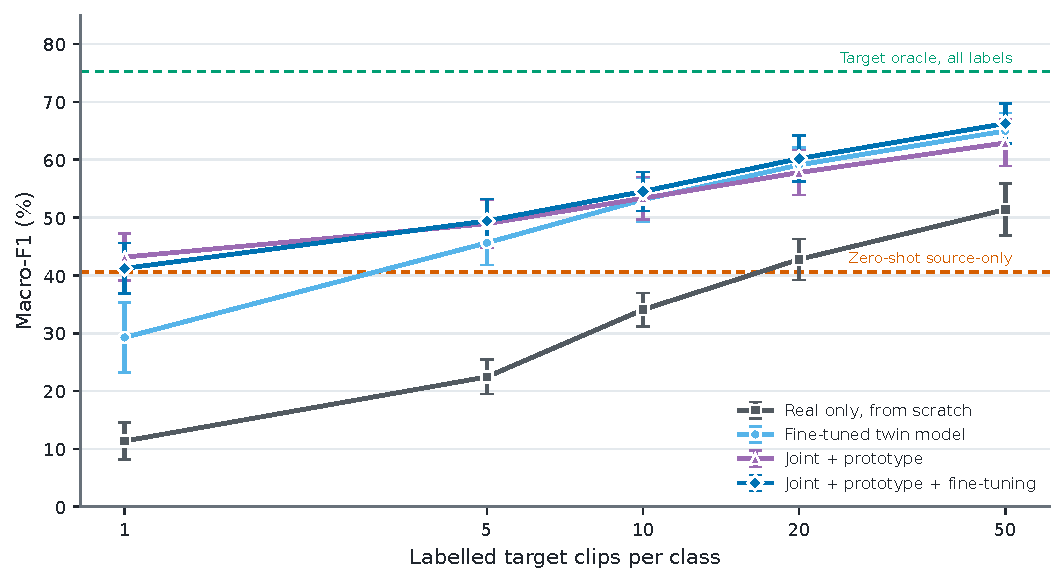
\includegraphics[width=.82\textwidth]{figures/paper_ready/few_shot.pdf}
  \caption{Macro-F1 against the number of labelled physical clips per class.}
  \label{fig:fewshot}
\end{figure}

\section{Discussion}
\label{sec:discussion}

\subsection{Digital twin role}

The results separate two roles that a digital twin could play. As a
replacement for physical data it fails in this benchmark: a recogniser that is
as good as a physically trained one inside the twin loses about 35 points of
macro-\ac{f1} on real workers, and no unsupervised method recovers them. As a
source of pretraining and of additional labelled examples it succeeds, since
it cuts the physical labels needed for a given accuracy by a factor of five to
twenty. The gap analysis explains this contrast. The obvious differences
between the domains, which are heading, segment boundaries, class proportions,
handedness and sensor jitter, are either removed by preprocessing or shown by
intervention not to limit recognition. What remains is a per-class difference
in execution that unlabelled target data cannot reveal, because aligning the
overall feature distribution says nothing about which physical motion
corresponds to which virtual action. A few labelled physical clips per class
supply exactly that correspondence, which is why they are so effective once
the twin has provided the rest of the representation.

\subsection{Implications for deployment}

For a new collaborative workcell these findings suggest a simple procedure.
The recogniser is first trained on the digital twin, after which a
class-balanced calibration set of a few clips per action is recorded with the
target workforce. With one to five clips per class the twin should be kept in
training together with the calibration clips and a class-prototype term, and
from about ten clips per class a final fine-tuning stage on the physical clips
alone should follow. In this benchmark thirteen physical clips already match
two hundred and sixty clips used without the twin, and fifty clips per class
reach $88\%$ of the oracle macro-\ac{f1} with about $18\%$ of its labels. The
oracle should be read as an upper bound and not as an operational
requirement, and the acceptable budget depends on the cost of
misrecognising each action in the assistance policy.

\subsection{Threats to validity}

The study uses one virtual and physical dataset pair, one backbone and one
action taxonomy, and its conclusions describe this transfer setting rather
than every digital twin. The label savings depend on how support clips are
sampled, and our class-balanced sampling may be optimistic compared with
opportunistic annotation on a production line. The diagnostic interventions
were run with a single seed and the pairwise tests are not corrected for
multiple comparisons. The evaluation concerns recognition on held-out workers
and not closed-loop robot assistance, so improved macro-\ac{f1} does not by
itself establish safer or more efficient collaboration. Finally, the
\ac{inharddt} participants differ from the \ac{inhard} workers, so the
domain gap mixes the effect of the virtual environment with that of the worker
population, and a study in which the same people work in both settings would
be needed to separate the two.

\section{Conclusion}
\label{sec:conclusion}

Collecting labelled recordings from every worker and workcell is costly, which
makes digital-twin data attractive for industrial action recognition. However,
virtual recordings may not represent how workers move and interact with
equipment in a physical cell. We examined this transfer problem using
\ac{inharddt} as the source and \ac{inhard} as the target, and proposed a
label-efficient strategy that trains on the twin and a few labelled physical
clips with a class-prototype term, then fine-tunes. With a shared \ac{ctrgcn}
backbone, we compared source-only transfer and unsupervised adaptation under
four subject-disjoint folds and three random seeds, then evaluated few-shot
adaptation with target labels while keeping test workers held out.

The results show that the tested unsupervised methods did not reliably improve
zero-shot performance: source-only transfer reached $40.59\%$ macro-\ac{f1},
compared with $39.34\%$ for \ac{tcmmd}. With target labels, a model initialised
on the digital twin matched the macro-\ac{f1} of a model trained on physical
clips alone while using five to twenty times fewer labelled clips, and the
class-prototype term added a significant gain at one and five clips per class.
The proposed strategy achieved the highest mean macro-\ac{f1} among the
label-efficient strategies from five clips per class upwards and reached
$66.27\%$ with 50 labelled target clips per class. %, below the $75.22\%$ target
% oracle. 
The gains as the label budget
increased show that digital-twin pretraining can provide a strong starting
point for adaptation, while physical labels remain important.

Further work
should test this finding across more workcells, worker groups, and sensing
conditions, and evaluate whether recognition gains support calibrated,
risk-sensitive robot assistance.

\section*{Funding Statement}

The authors received no financial support for the research, authorship, and/or
publication of this article.

% \section*{Data availability}

% \ac{inharddt} and \ac{inhard} are available from Zenodo records 7644247 and
% 4003541~\cite{dallel2023dataset,dallel2020inhard}. The preprocessing code,
% training code, saved per-run predictions and analysis notebooks will be made
% available upon publication.

\bibliography{references}

\clearpage
\thispagestyle{empty}
\begin{center}
  \textbf{For Table of Contents Only}\\[1em]
  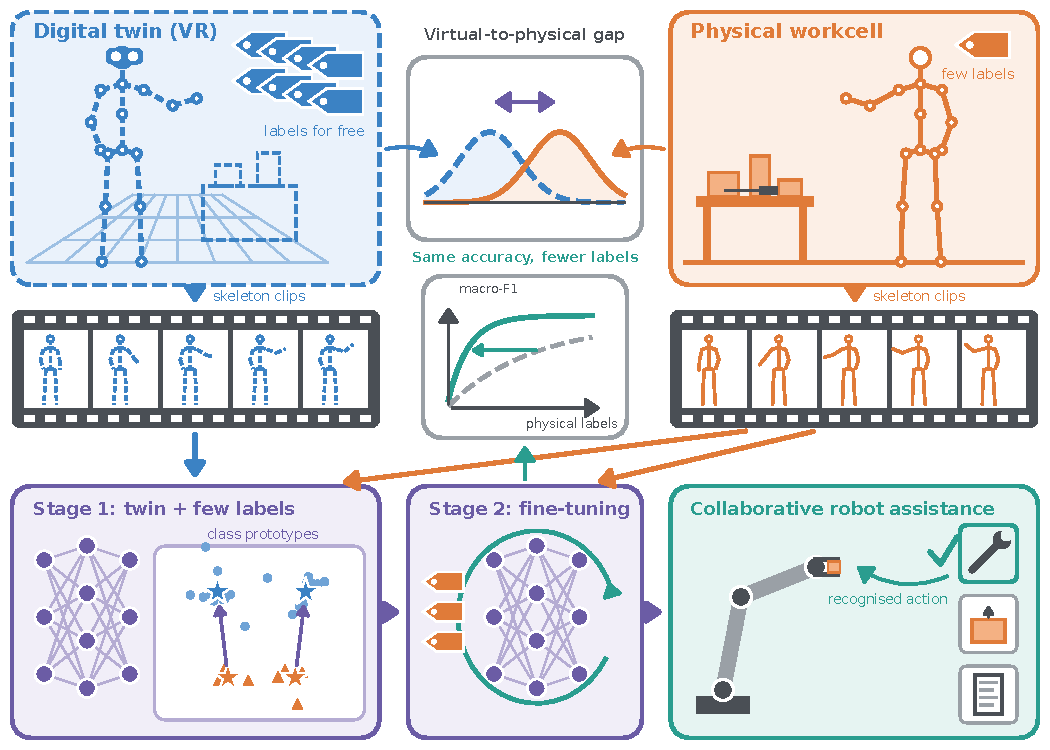
\includegraphics[width=\textwidth]{graphical_abstract.pdf}
\end{center}
\end{document}
